\chapter{Implémetation et Exploitation}

\section*{Introduction}%
\addcontentsline{toc}{section}{\numberline{}Introduction}%
Ce chapitre est dédié à l’implémentation du système et la présentation des résultats obtenus. Nous présenterons les ETL conçus, l’entrepôt de données et les magasins de données, les cubes d’analyse conçus et quelques tableaux de bords réalisés. 

\section{Implémetation du Datawarehouse}
\subsection{Choix de l'Outil d'Implémetation}
Puisque nous allons travailler avec de données structures nous utiliserons un SGBD\footnote{Systeme de Gestion des Bases de Donnees} SQL. Le tableau \ref{tab:comparaisonsgbd} montre une comparaison entre les SQBD SQL les plus populaires.
\begin{table}[H]
    \centering
    \caption{Comparaison des SGBD.}
    \begin{tabular}[t]{|p{3cm}|p{4.5cm}|p{3cm}|p{1.5cm}|p{2cm}|} 
        \hline
        \textbf{SGBD} & \textbf{Structure} & \textbf{Licence} & \textbf{Docs} & \textbf{Difficile } \\
        \hline\hline
        MySQL & SQL & Publique & ++ & + \\
        \hline
        PostgreSQL & SQL et relationnel-objet & Open source & ++ & ++ \\
        \hline
        Oracle & Multi SQL et SQL & Privée & +++ & +++ \\
        \hline
        MSSQL Server & T-SQL & Privée & +++ & ++ \\
        \hline\hline
    \end{tabular}
    \label{tab:comparaisonsgbd}
\end{table}%
T-SQL représente Transact-SQL est une façon de faire du SQL qui nous permet de faire des requêtes complexes et permet aussi de faire des procédures stockes, ce qui est très important pour notre projet. De ce fait nous avons décidée d’utiliser la SGBD \textbf{MSSQL Server}.
\subsection{Installation de SQL Server 2019}  

Les captures suivantes montrent les étapes importantes pendant l’installation de SQL Server 2019, la dernière version de SQL Server. Après lancement de l’installation, sur le volet gauche on clique sur Installation ou on tombe sur une fenêtre comme la figure \ref{fig:choisirservice} qui permet de choisir les service a installer.
\begin{figure}[H]
    \centering
    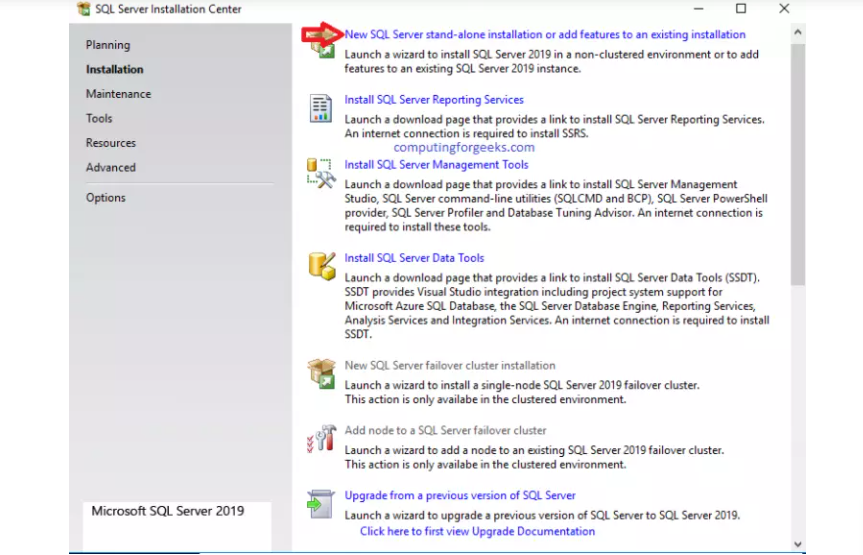
\includegraphics[width=12cm]{choisirservice}
    \caption{SQL Server : Choix du Service a Installer}
    \label{fig:choisirservice}
\end{figure} 

Ayant choisi d’installer une nouvelle instance de SQL Server la capture dans l’image \ref{fig:chooseedition} montre la page pour choisir l’édition à installer. On choisit l’édition Developer puisque c’est l’édition gratuite de SQL Server.

\begin{figure}[H]
    \centering
    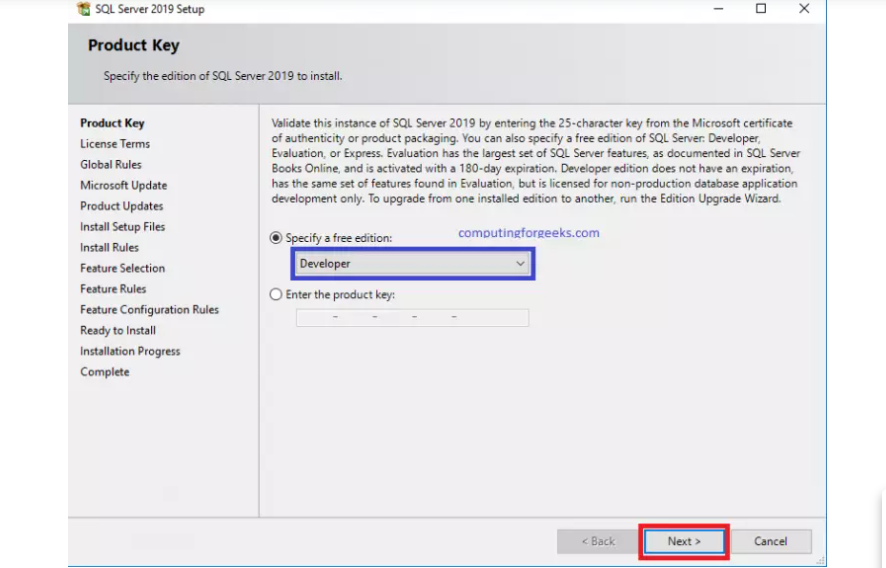
\includegraphics[width=12cm]{chooseedition}
    \caption{SQL Server : Choix de l’édition a Installer}
    \label{fig:chooseedition}
\end{figure} 

Ensuite on accepte les termes et conditions, puis on choisit si on veut les mises à jour ou pas. Ensuite il faudra choisir les fonctionnalités à installer comme dans la figure \ref{fig:featureselection}


\begin{figure}[H]
    \centering
    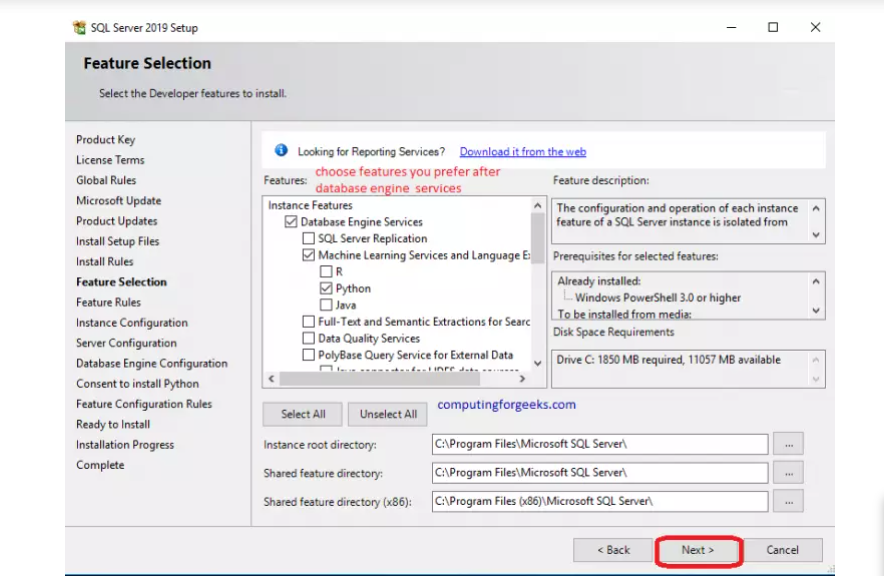
\includegraphics[width=12cm]{featureselection}
    \caption{SQL Server : Choix des fonctionnalités à installer}
    \label{fig:featureselection}
\end{figure}

La figure \ref{fig:instanceconfig} démontre la page de configuration de l’instance à installer ou on donne le nom et l’ID de l’instance. 

\begin{figure}[H]
    \centering
    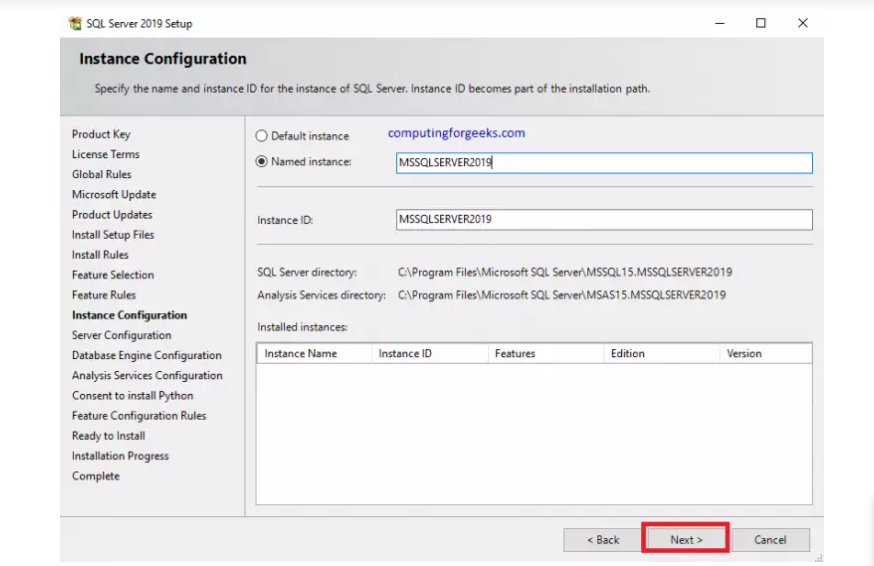
\includegraphics[width=12cm]{instanceconfig}
    \caption{SQL Server : Configuration de l'instance}
    \label{fig:instanceconfig}
\end{figure}

La prochaine étape c’est la configuration du serveur, ensuite on configure le moteur de bases de données comme dans la figur\ref{fig:dbengineconfig}.

\begin{figure}[H]
    \centering
    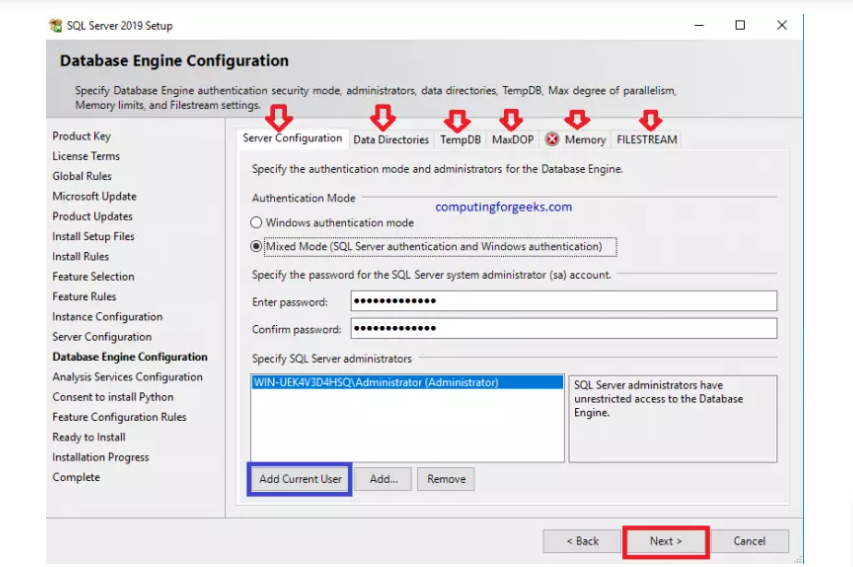
\includegraphics[width=12cm]{dbengineconfig}
    \caption{SQL Server : Configuration du moteur de  bases de données}
    \label{fig:dbengineconfig}
\end{figure}

Ensuite une nous présente un resumé de l'installation et on lance l'installation.


\subsection{Creation des Bases de donnees}
\subsubsection{Base de Données STAGING}
La STAGING c’est la base de données de préparation pour le datawarehouse, ainsi c’est dans la STAGING que nous allons charger nos données provenant de l’ERP et de là nous allons alimenter la DATAWAREHOUSE ainsi que les DATAMARTS. La figure \ref{fig:capturestaging} est une capture des tables dans la STAGING. 

\begin{figure}[H]
    \centering
    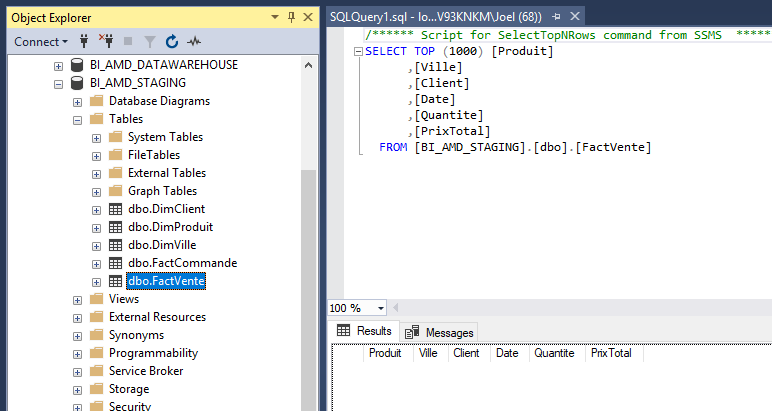
\includegraphics[width=\textwidth]{capturestaging}
    \caption{Base de Données STAGING}
    \label{fig:capturestaging}
\end{figure}


\subsubsection{Base de Données DATAWAREHOUSE}

De la STAGING, la DATAWAREHOUSE est alimentée. Ceci est faite en exécutant la procédure stockée appropriée. La figure \ref{fig:capturedwh} montre une capture de la DATAWAREHOUSE et ses tables.

\begin{figure}[H]
    \centering
    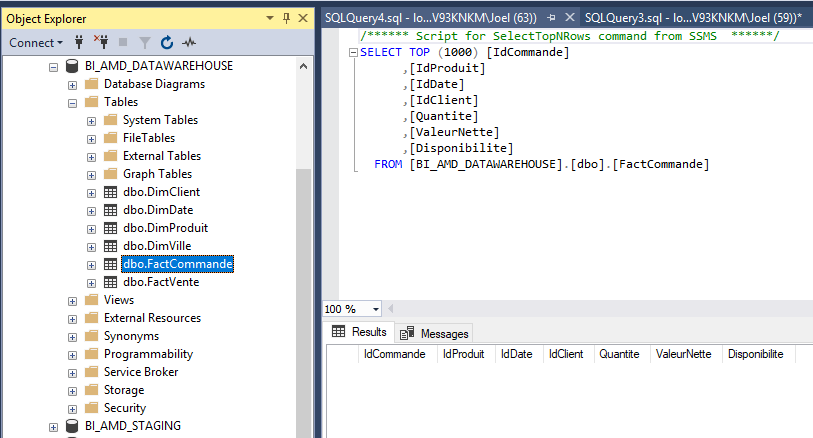
\includegraphics[width=\textwidth]{capturedwh}
    \caption{Base de Données DATAWAREHOUSE}
    \label{fig:capturedwh}
\end{figure}
 
\subsubsection{Base de Données DATAMART\_VENTE}

De la même façon que la DATAWAREHOUSE est alimentée en utilisant une procédure stockée, les datamarts aussi le sont mais cette fois ci à partir du DATAWAREHOUSE et non de la STAGING. La figure \ref{fig:capturedatamartvente} montre la DATAMART\_VENTE et ses tables qui correspondent exactement aux tables dans la DATAWAREHOUSE.

\begin{figure}[H]
    \centering
    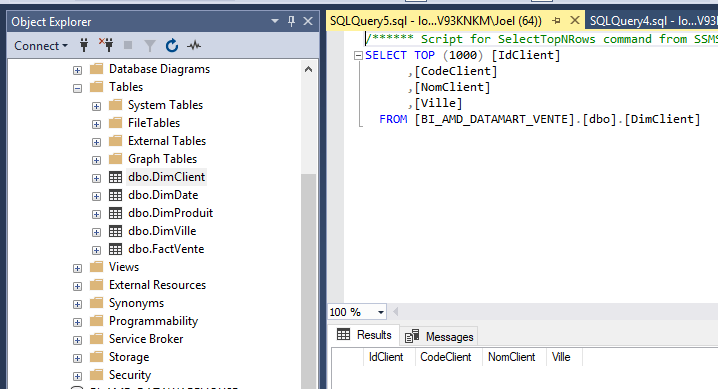
\includegraphics[width=\textwidth]{capturedatamartvente}
    \caption{Base de Données DATAMART\_VENTE}
    \label{fig:capturedatamartvente}
\end{figure}

\subsubsection{Base de Données DATAMART\_COMMANDE}

\begin{figure}[H]
    \centering
    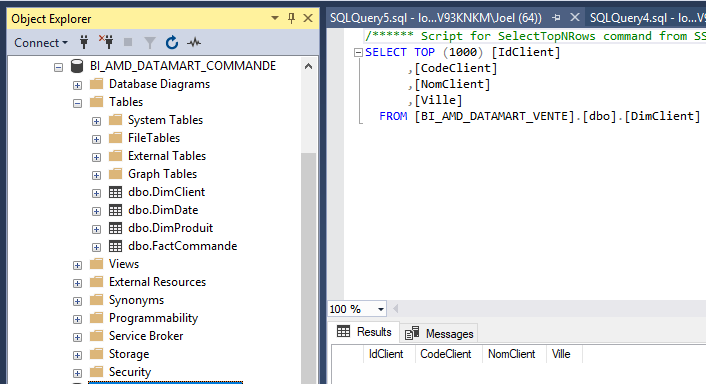
\includegraphics[width=\textwidth]{capturedatamartcommande}
    \caption{Base de Données DATAMART\_COMMANDE}
    \label{fig:capturedatamartcommande}
\end{figure}

\section{Implémetation des ETL}

\subsection{Choix de l'Outil d'Implémetation}
Puisque nous avons choisi de développer le système de B.I. de bout en bout, on a décidé d’utiliser l’ensemble d’outils de Microsoft pour le faire. Dans cette suite d’outils, pour faire les ETL on a SSIS (SQL Server Integration Services). C’est un outil très riche qui nous permettra de mettre sur pied des connexions a nos données sur l’ERP Sage et facilement les charger dans la datawarehouse. 

\subsection{Installation de SQL Server Integration Services}
\subsubsection{Téléchargement de SSDT}
Les étapes suivantes consistent à télécharger SSIS via les outils SSDT. 
\begin{itemize}
    \item Ouvrez le centre d'installation de SQL Server ;
    \item Cliquez sur Installation dans le menu de gauche ;
    \item Cliquez sur \textit{Install SQL Server Data Tools} pour parcourir une page Web de téléchargement ;
    \item Une fois la page de téléchargement ouverte, cliquez sur le lien de téléchargement SSDT ;
    \item  Vérifiez le fichier d'installation SSDT dans le dossier de téléchargement. Le nom est \textit{SSDT-Setup-ENU}.
\end{itemize} 

\subsubsection{Installation de SSIS}
Les étapes suivantes consistent à installer SSIS via les outils SSDT. 
\begin{itemize}
    \item Ouvrez le fichier d'installation \textit{SSDT-Setup-ENU}.
    \item La page d'accueil de Microsoft SQL Server Data Tools s'affiche, puis cliquez sur le bouton Suivant pour commencer les étapes d'installation
    \item Sur la zone de liste déroulante affichera les options d'installation dans l'instance Visual Studio actuelle ou existante ou une nouvelle instance Visual Studio. Si vous choisissez une nouvelle instance, nommez la.
    \item Pour installer SSIS , vérifiez les services d'intégration SQL Server, puis cliquez sur le bouton Installer comme suit.
    \begin{figure}[H]
        \centering
        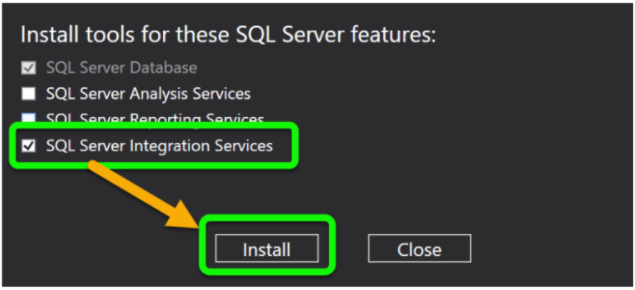
\includegraphics[width=\textwidth]{checkssis}
        \caption{Vérifiez l'option SQL Server Integration Services}
        \label{fig:checkssis}
    \end{figure}
    \item  Avant de cliquer sur le bouton Installer, assurez-vous que Microsoft Visual Studio n'est pas ouvert et connecté à Internet, sinon un message d'erreur apparaîtra.
    \item La progression du téléchargement et de l'installation apparaîtra comme suit:
    
    \begin{figure}[H]
        \centering
        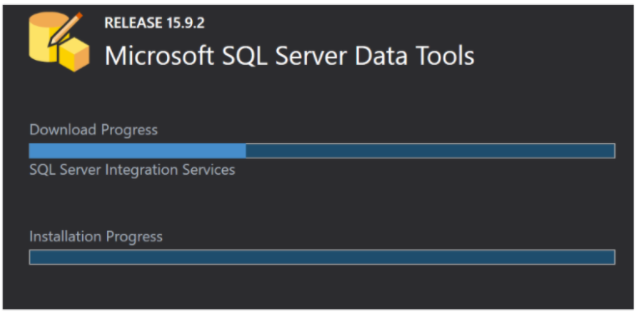
\includegraphics[width=\textwidth]{ssisprogress}
        \caption{Progression du téléchargement et de l'installation de SSIS}
        \label{fig:ssisprogress}
    \end{figure}
    \item Lorsque la progression est terminée, l'ordinateur redémarrera.
    \item Une fois terminé, les services d'intégration seront disponibles dans le projet d'entreprise Visual Studio comme indiqué ci-dessous: 
    \begin{figure}[H]
        \centering
        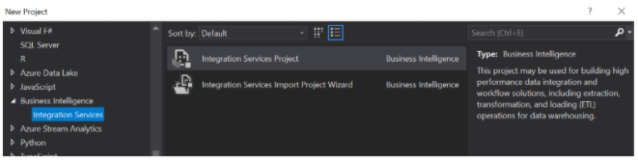
\includegraphics[width=\textwidth]{ssisproject}
        \caption{Le projet des services d'intégration}
        \label{fig:ssisproject}
    \end{figure}
\end{itemize} 

\subsection{Creation des ETL}
\subsubsection{ETL de chargement dans la base STAGING}

\begin{figure}[H]
    \centering
    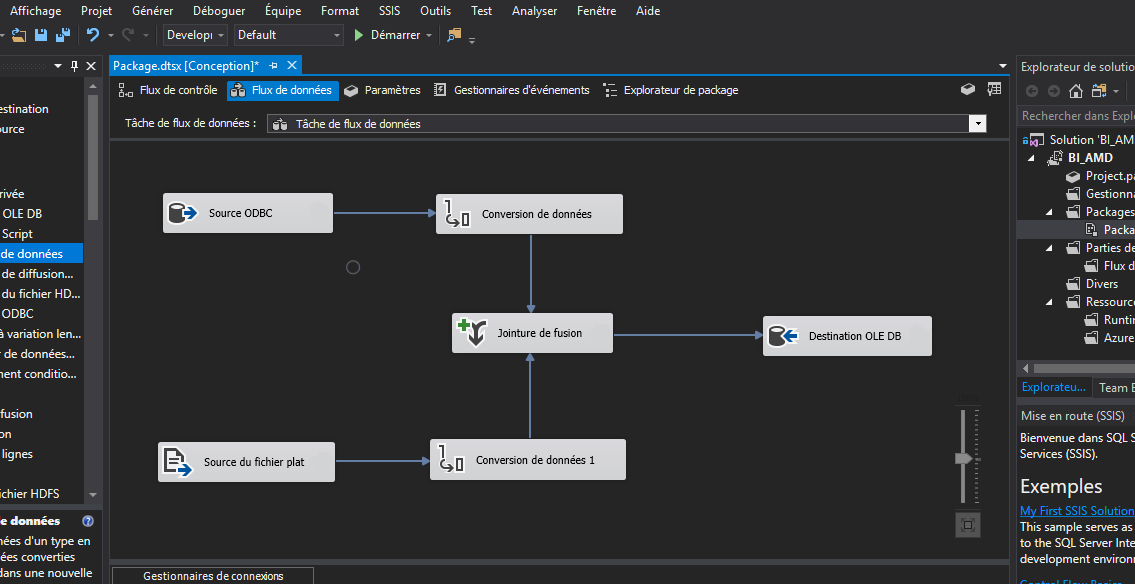
\includegraphics[width=\textwidth]{ssisetlstaging}
    \caption{L'ETL de chargement de la STAGING}
    \label{fig:ssisetlstaging}
\end{figure}

\subsubsection{ETL d'alimentation de la base DATAWAREHOUSE}
Comme indiqué plus haut elle ne comporte qu'une tache d'execution de requêtes SQL.

\begin{figure}[H]
    \centering
    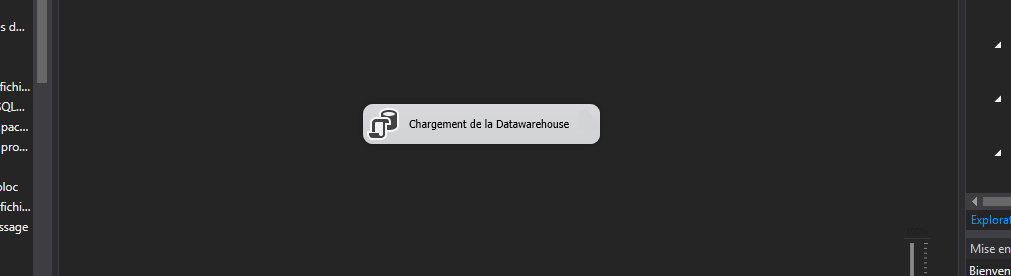
\includegraphics[width=\textwidth]{ssisetldatawarehouse}
    \caption{L'ETL de chargement de la DATAWAREHOUSE}
    \label{fig:ssisetldatawarehouse}
\end{figure}

\subsubsection{ETL d'alimentation de la base DATAMART\_VENTE}
Comme pour la DATAWAREHOUSE elle ne comporte qu'une tache d'execution de requêtes SQL.
\begin{figure}[H]
    \centering
    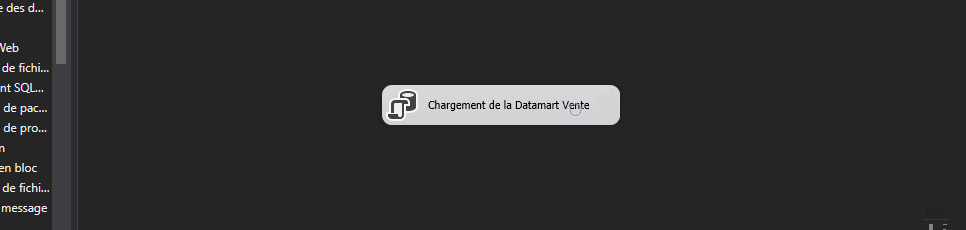
\includegraphics[width=\textwidth]{ssisetldatamartvente}
    \caption{L'ETL de chargement de la DATAMART\_VENTE}
    \label{fig:ssisetldatamartvente}
\end{figure}

\subsubsection{ETL d'alimentation de la base DATAMART\_COMMANDE}
Comme pour la DATAWAREHOUSE elle ne comporte qu'une tache d'execution de requêtes SQL.
\begin{figure}[H]
    \centering
    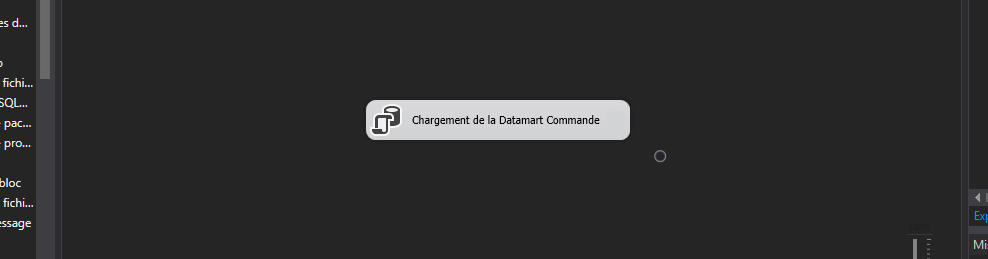
\includegraphics[width=\textwidth]{ssisetldatamartcommande}
    \caption{L'ETL de chargement de la DATAMART\_COMMANDE}
    \label{fig:ssisetldatamartcommande}
\end{figure}


\section{Chargement des Données}
\subsection{Utilisation du Connecteur ODBC}
La capture dans la figure \ref{fig:fenetreconnexionodbc} montre la fenêtre de configuration de la connexion a notre ERP.
\begin{figure}[H]
    \centering
    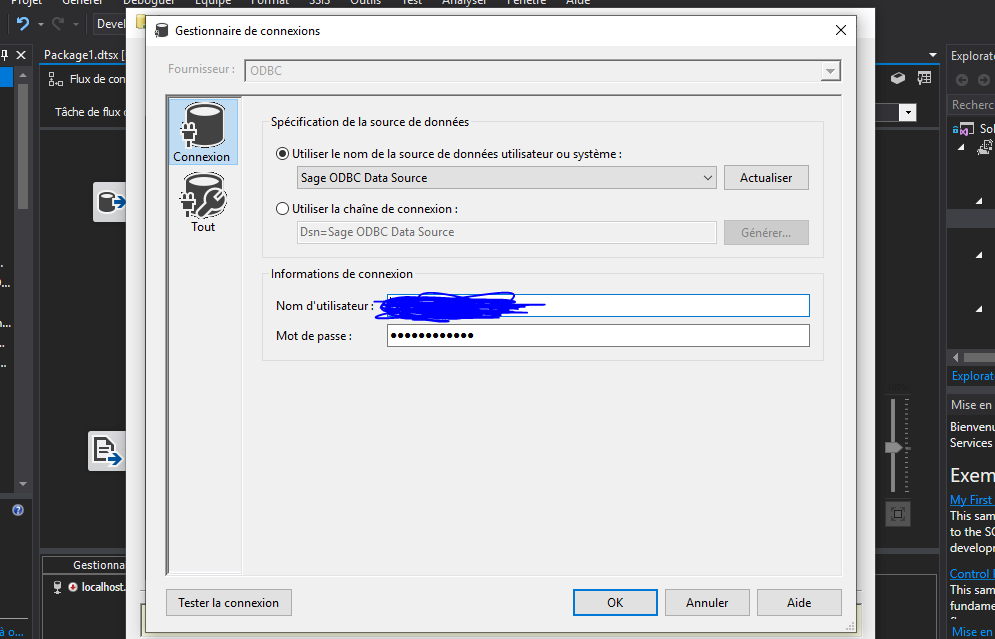
\includegraphics[width=\textwidth]{fenetreconnexionodbc}
    \caption{Fenêtre de configuration de la source ODBC}
    \label{fig:fenetreconnexionodbc}
\end{figure}

\subsection{A partir de fichiers plats}
La capture dans la figure \ref{fig:fenetreconnexionfichierplat} montre la fenêtre de configuration de la connexion a notre fichier plat.
\begin{figure}[H]
    \centering
    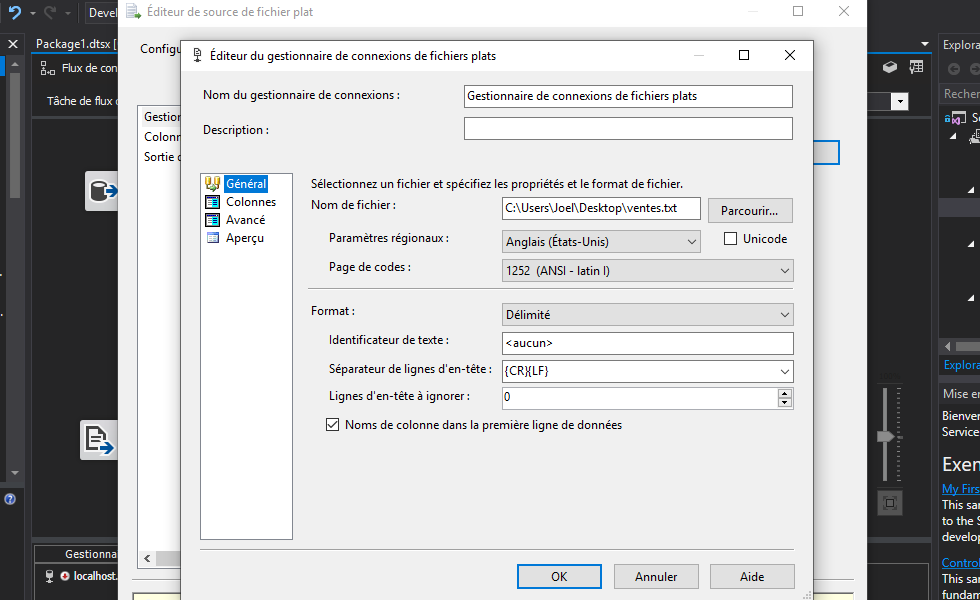
\includegraphics[width=\textwidth]{fenetreconnexionfichierplat}
    \caption{Fenêtre de configuration de la source fichier plat}
    \label{fig:fenetreconnexionfichierplat}
\end{figure}

\section{Exploitation de la Datawarehouse}
\subsection{Choix d'outil d'exploitation}
Pour exploiter notre Datawarehouse nous aurons besoin d’analyser nos données puis de les visualiser. De nombreux outils existent d’analyse et de visualisation mais nous avons opté pour Power B.I. grâce a sa compatibilité avec multiple types de sources de donnes et le fait qu’il permet de faire de l’analyse dans le même outil. Aussi l’outil a une version mobile qui permet l’utilisation de notre système même par votre téléphone mobile rendant ainsi l’accessibilité plus grande. 
\subsection{Analyse avec Power BI}
En effet Power B.I. depuis 2017 intègre un composant pour analyser et former des cubes de données avant de passer à leurs visualisations. Nous profitons de cet avantage pour nous passer de l’utilisation d’un outil supplémentaire. La capture dans la figure \ref{fig:powerquerydatamanip} montre la manipulation des données dans \textbf{PowerQuery}, le composant de Power B.I. qui permet de faire la manipulation des données en fonction des objectifs de l’analyse.
\begin{figure}[H]
    \centering
    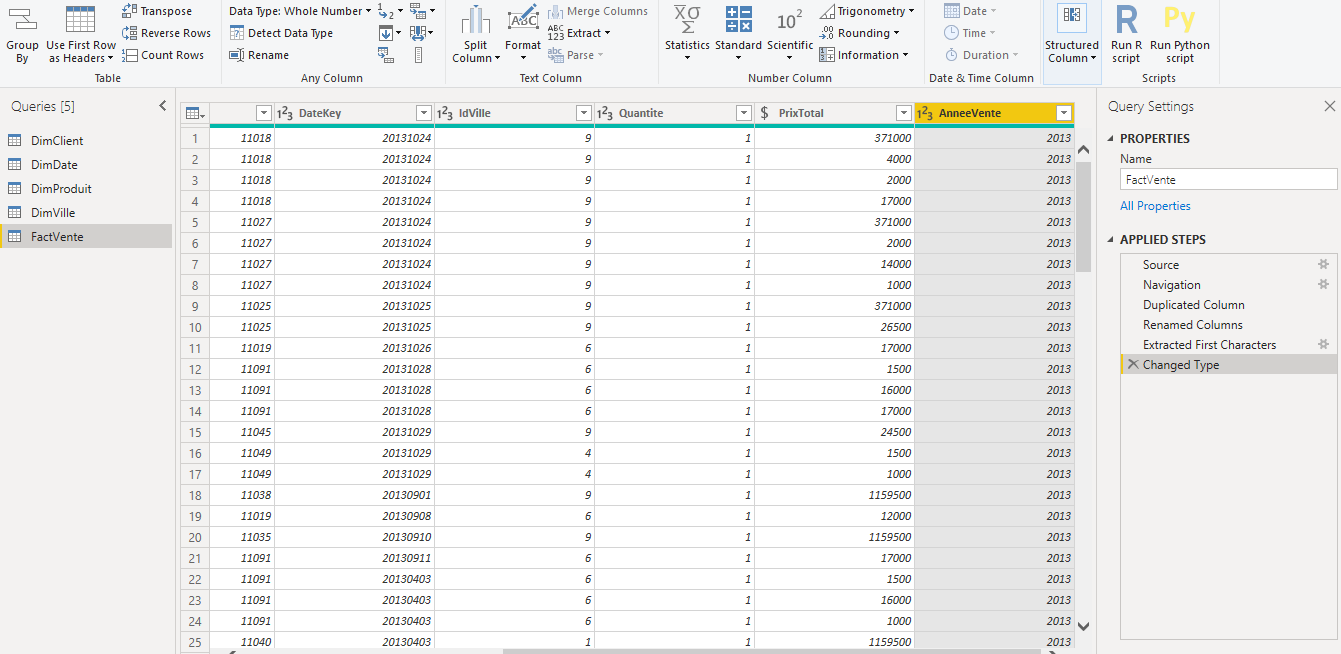
\includegraphics[width=\textwidth]{powerquerydatamanip}
    \caption{Manipulation des données avec PowerQuery}
    \label{fig:powerquerydatamanip}
\end{figure}
Après avoir manipulé nos données et atteint nos objectifs nous commençons donc à former nos cubes de données qui permettront la mise en place des tableaux de bord. La capture dans la figure \ref{fig:powerbianalysisvente} montre notre cube du Datamart Vente fait dans Power B.I.

\begin{figure}[H]
    \centering
    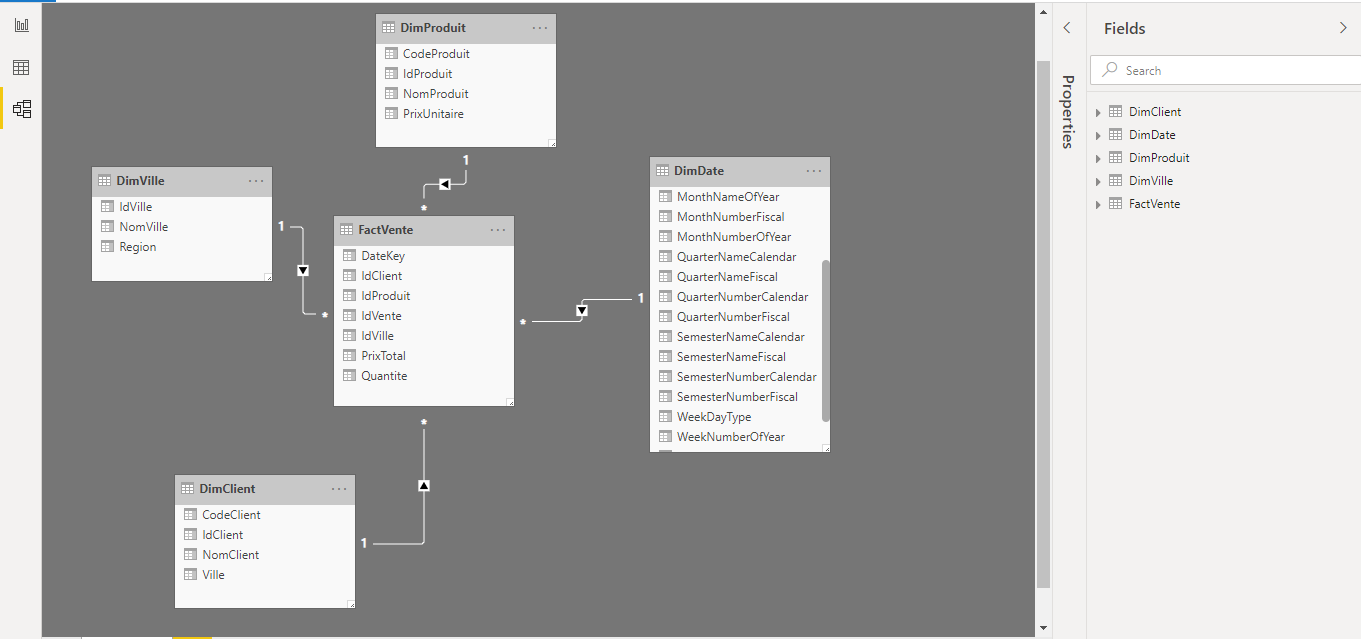
\includegraphics[width=\textwidth]{powerbianalysisvente}
    \caption{Cube du datamart Vente dans Power B.I.}
    \label{fig:powerbianalysisvente}
\end{figure}

\subsection{Visualisation avec Power BI}
Ici nous présentons les résultats obtenus après la conception des tableaux de bords sur power B.I. La figure \ref{fig:dashboard1} montre plusieurs aspects sur les relations entre les prix et les ventes proposant des prix optimaux pour chaque produit.
\begin{figure}[H]
    \centering
    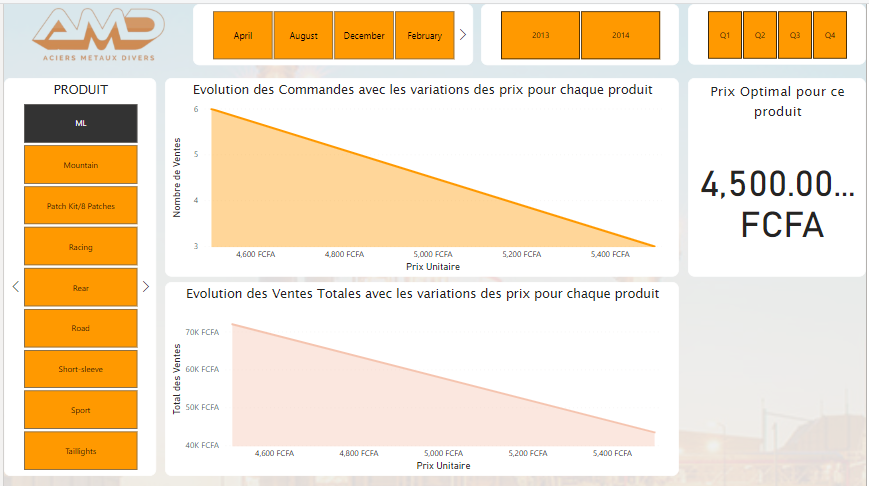
\includegraphics[width=\textwidth]{dashboard1}
    \caption{Tableau de bord proposant un prix optimal}
    \label{fig:dashboard1}
\end{figure}

La figure \ref{fig:dashboard2} montre les pourcentages des ventes totales des differents prix pour un produit en particulier. On peut donc clairement voir le prix avec leque on vend le plus.
\begin{figure}[H]
    \centering
    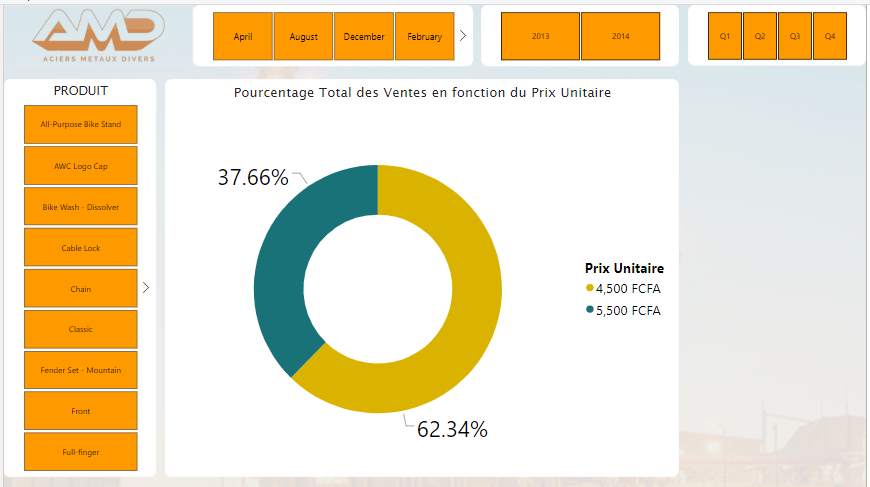
\includegraphics[width=\textwidth]{dashboard2}
    \caption{Tableau de bord montrant le ratio entre les prix et les ventes totales}
    \label{fig:dashboard2}
\end{figure}

\subsection{Déploiement de la solution}
Nous allons déployer notre solution et la partager aux utilisateurs à l'aide Power B.I. Service, l'outil de déploiement de Power B.I. Il permet à l'utilisateur de visualiser ses tableaux de bords à partir de son navigateur web et aussi à partir de son téléphone mobile grâce à l'application mobile de Power B.I. La figure \ref{fig:powerbideploy} montre une architecture du déploiement des rapports sur Power B.I. Service.

\begin{figure}[H]
    \centering
    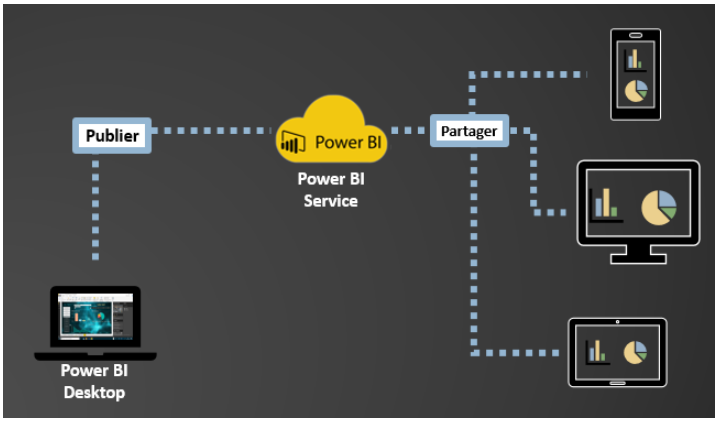
\includegraphics[width=\textwidth]{powerbideploy}
    \caption{Architecture de déploiement sur Power B.I. Service}
    \label{fig:powerbideploy}
\end{figure}

\section*{Conclusion}%
\addcontentsline{toc}{section}{\numberline{}Conclusion}%
Ce chapitre avait pour objectif de présenter l’implémentation des différentes parties de notre solution ainsi que le résultat final du projet. Il constitue le dernier chapitre de ce document. Nous pouvons maintenant conclure et parler des perspectives.

